\scanpage{234}
\uline{\mspage{1}}
\figure{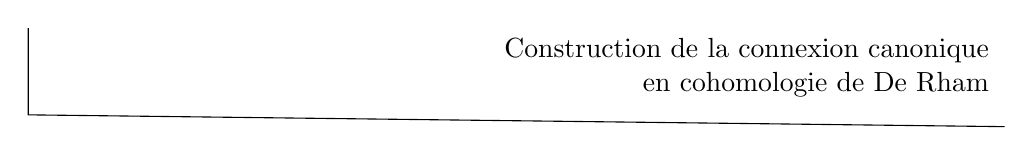
\begin{tikzpicture}[baseline=(n.base)]\node(n)[align=right,text width=12cm] at (0,0){Construction de la connexion canonique\\en cohomologie de De Rham};\draw (-6.2,0.5)--(-6.2,-0.6)--(6.2,-0.75);\end{tikzpicture}}

\diagram{\begin{tikzcd}[column sep=large]
X_0\arrow[d,"f_0"]&X'\arrow[d,"f'"]&X''\arrow[dl,"f''"]\\
T_0\arrow[r,hook,no head,"\substack{\text{immersion}\\1\text{-nilpotente}}"']&T
\end{tikzcd}}
\margin{schéma relatif \unsure{formellt.} lisse}
\margin{\figure{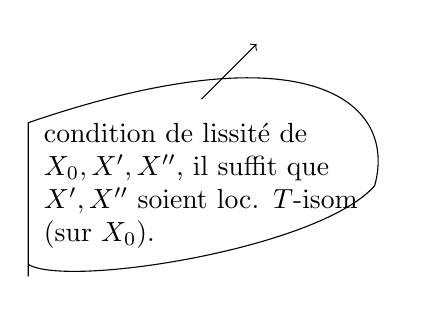
\begin{tikzpicture}[baseline=(n.base)]\node(n)[text width=4cm,align=left] at (0,0){\unsure{condition} de lissité \inserted{de $X_0,X',X''$}, \unsure{il} suffit que $X',X''$ soient loc. $T$-isom (sur $X_0$).};\draw (-2.2,-1.15)--(-2.2,0.8) .. controls (1.3,2) and (2.5,1.1) .. (2.2,0) .. controls (1.5,-0.8) and (-1.7,-1.3) .. (-2.2,-1);\draw[->] (0,1.1)--(0.7,1.8);\end{tikzpicture}}}
\[
T_0=V(\underline{I})
\]
\[
X'\mathbin{\times}_T T_0\xrightarrow{\sim}X_0\qquad
X''\mathbin{\times}_T T_0\simeq X_0
\]
$X',X''$ deux prolongements lisses de $X_0/T_0$ sur $T$.

\diagram{\begin{array}{lll}
\mathcal P&\text{faisceau sur esp }X_0\text{ des germes des}&T\text{-isom }X'\to X''\\
\mathcal G&\rule{8cm}{0.4pt}&T\text{-autom }X''\to X''
\end{array}}
alors
\[
\mathcal G\simeq\operatorname{Hom}(\Omega^1_{X_0/T_0},f_0^{\unsure{*}}(I))
=\unsure{\mathcal T}_{X_0/T_0}\otimes f_0^{\unsure{*}}(\underline I)
\]
$\mathcal P$ un \inserted{$\mathcal G$-torseur à droite} [faisceau principal homogène \inserted{à droite} sur $\mathcal G$.]

\diagram{\begin{tikzcd}
\mathcal P\mathbin{\times}\Omega^\bullet_{X'/T}\arrow[r]&\Omega^\bullet_{X''/T}
\end{tikzcd}}
i.e.
\diagram{\begin{tikzcd}
\mathcal P\arrow[r,"u"]&\underline{\operatorname{Isom}\text{ de complexes}}(\Omega^\bullet_{X'/T},\Omega^\bullet_{X''/T})
\end{tikzcd}}
\[
\subset Z^0\underline{\operatorname{Hom}}^\bullet(\Omega^\bullet_{X'/T},\Omega^\bullet_{X''/T})
\]
\diagram{\begin{tikzcd}
\mathcal G\arrow[r,"v"]&\underline{\unsure{\operatorname{Aut}}\text{ de complexes}}(\Omega^\bullet_{X''/T})
\end{tikzcd}}
\[
\subset Z^0\underline{\operatorname{Hom}}^\bullet(\Omega^\bullet_{X''/T},\Omega^\bullet_{X''/T})
\]
\diagram{\begin{tikzcd}
\mathcal G\arrow[r,"k"]&\underline{\operatorname{Hom}}^{(-1)}(\underline{\Omega}^\bullet_{X''/T},\Omega^\bullet_{X''/T})
\end{tikzcd}}
par procédés antérieurs

On a
\[
\left\{\begin{aligned}
u(pg)&=u(p)v(g)\qquad&\text{si }p&\in\Gamma(U,\mathcal P)\\
&&g&\in\Gamma(U,\mathcal G)\\
v(g)-\mathrm{id}&=dk(g)+k(g)d
\end{aligned}\right.
\]
\margin{233}
